\section{Delegation}

In this section we describe the delegation mechanism for each account defined in section \ref{sec:account}. Specifically, we define the structure of the certificates used for delegating the stake of a pointer account, as well as the structure of the delegation pointers in a pointer account. The stake in an enterprise account is by definition not used in the Proof-of-Stake protocol, although if it were used then the delegation would be exactly the same as in the pointer accounts. Finally, we also describe the rules for chain delegation.

\subsection{Delegation certificate}

Delegation is achieved by linking an account with a staking key. For pointer accounts, this link is achieved by pointing the account to a delegation certificate. That certificate can be part of a transaction and is thus posted on the blockchain, i.e. it is a \textbf{heavyweight} certificate.

Posting a heavyweight certificate for account $\alpha$ is equivalent to posting a transaction that contains the certificate as part of its data. Therefore, the account that the certificate pertains to and the account that posts it might be completely separate. For example, a user might create a certificate for an account $\alpha_0$ that he owns and post it by creating a transaction that transfers the balance from account $\alpha_1$ to $\alpha_2$.

The first part of the certificate is the delegate key which is defined below.

\begin{defn}[Delegate key]\label{def:delegate_key}
The delegate key $K_D$ of $\alpha$ is a staking key ${K^s}'$, which takes part in the Proof-of-Stake protocol on behalf of an account $\alpha$ that has delegated to it.
\end{defn}

The second part is the staking key $K^s$ that the certificate pertains to. Specifically, $K^s$ is included here in plaintext and the certificate defines that all stake managed by $K^s$, either directly in a base account or indirectly in a pointer account, is delegated to $D$.

The third part of a heavyweight certificate is the chain rule $c$. $c$ is 1 bit that defines if chain delegation is allowed for all stake that the certificate pertains to. In principle the delegate key in a certificate that does not allow chain delegation should be the staking key of a stake pool. The maximum length of a delegation chain using heavyweight certificates is 3. We define chain delegation below.

\begin{defn}[Chain delegation]\label{def:chain_delegation}
Chain delegation is the ability of a staking key to issue a delegation certificate for stake that has been delegated to it.
\end{defn}

For example, suppose two heavyweight certificates $c_0, c_1$ and two accounts $\alpha_0, \alpha_1$ that point to $c_0, c_1$ respectively. Also suppose that although the delegate key for both certificates is ${K^s}'$, $c_0$ allows chain delegation whereas $c_1$ does not. ${K^s}'$ then issues a heavyweight certificate for a staking key ${K^s}''$. In this case, if the stake of $\alpha_0$ is chosen as a slot leader, then ${K^s}''$ can create the valid block. However, if the stake for $\alpha_1$ is chosen, then ${K^s}''$ does not have the staking rights and ${K^s}'$ must create a block instead.

The final part of the certificate is a signature created by the staking key $K^s$. The signature is applied on all previous parts of the certificate and is used to verify that the certificate is valid for the staking key $K^s$ that it pertains to.

If two conflicting certificates exist for the same stake, then the valid is the latest on the blockchain. For example, suppose the staking key $K^s_0$ of a base account $\alpha_0$. That key can issue two certificates $c_1, c_2$, where the valid one for the stake in $\alpha_0$ is the newest one, e.g. $c_2$. However, suppose a pointer account $\alpha_1$ that points to $c_1$. In that case, $c_1$ is still valid for the stake in $\alpha_1$.

A staking key can create a certificate which is not posted on the blockchain, i.e. a \textbf{lightweight} certificate. A lightweight certificate is given off-chain to the owner of the delegate key and is published if the stake that it pertains to is used to create a block. Chain delegation from a lightweight certificate is not allowed, although any staking key can create a lightweight certificate.

In a lightweight certificate there also exists a lightweight counter. This counter is used to identify the valid certificate among multiple lightweight ones. Specifically, if two lightweight certificates are presented for the same stake, then the valid is the one with the higher counter value. However, this rule applies only on chains of equal length, where the dispute is on the last block in the chain. In case a block is minted on top of the block under dispute, then the lightweight counter is no longer taken into account and the longest chain rule stands.

The structure of a heavyweight and a lightweight delegation certificate can be seen in Figures \ref{fig:certificate_v2} and \ref{fig:light_certificate_v2}.

\begin{figure}
  \begin{center}
    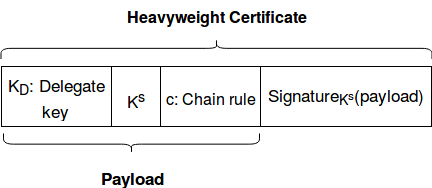
\includegraphics[width=340pt]{figures/certificate_v2.png}
  \end{center}
  \caption{The heavyweight delegation certificate.}
  \label{fig:certificate_v2}
\end{figure}

\begin{figure}
  \begin{center}
    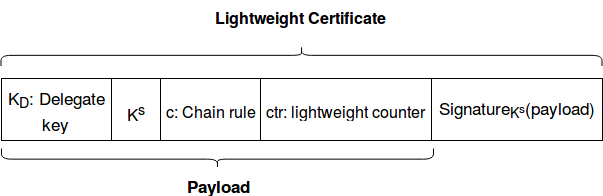
\includegraphics[width=340pt]{figures/light_certificate_v2.png}
  \end{center}
  \caption{The lightweight delegation certificate.}
  \label{fig:light_certificate_v2}
\end{figure}

\subsection{Base delegation}

As described in \ref{subsubsec:base_account_v2} a base account contains a delegation hash $dh$, which is the hash of a staking key $K^s$. Therefore, the stake in a base account is automatically controlled by $K^s$, i.e. $K^s$ can create a block for the stake in the account and the system can verify the eligibility of the key by comparing $dh$ to that key. Also $K^s$ can create and post a delegation certificate.

\subsubsection{Posting a heavyweight certificate}

A certificate is posted on the blockchain by creating a transaction that contains the certificate in its data. However, who creates this transaction and which money it pertains to is not always trivial.

One case is when the user $A$ expects some payment from another user $B$. In that case, $A$ can simply give the certificate to $B$ to include it in the payment transaction. However, it might be the case that the user wishes to post a certificate without waiting for a payment.

In this case, the user maintains a \textit{pocket} account, i.e. an account used solely for posting certificates. This is a $pointer$ account that contains a minimal amount of funds, enough for posting just a finite amount of certificates. The user keeps a \textit{pocket} account for each staking key that she manages. Therefore, when she wishes to post a certificate using a staking key $K^s_1$, she posts a transaction from the \textit{pocket} account ${\alpha}^p_1$ to ${\alpha}^p_2$, both of which are managed by the user and pertain to the staking key $K^s_1$.

\subsection{Pointer delegation}

Pointer delegation is the delegation of the stake in a pointer account. Specifically, the address in such account contains a delegation pointer. We define the delegation pointer below.

\begin{defn}[Delegation pointer]\label{def:delegation_pointer}
The delegation pointer $ptr$ is a tuple of two indexes, the index $b$ of a block in the blockchain and the index $x$ of a transaction in a block:

$ptr = (b, x)$.
\end{defn}

The staking key for the stake in a pointer address is found as follows. First, the transaction identified by the delegation pointer $ptr$ is found. If the transaction does not contain a valid certificate, then the stake is left un-delegated. Otherwise, delegation follows the rules defined in that transaction's certificate, i.e. the stake is delegated to the certificate's delegate key and the chain rule for the stake is the one defined in the certificate.
